\newcommand\pdescitemsep{-0.2em}
\section{Initial project description}

This project will attempt to develop an automatic system identification and controller tuning algorithm for use in EtherCAT servo drives using the CiA-402 communication protocol.
The project will be developed in a ROS2 environment. 
 
The EtherCAT connectivity will be handled be an open-source EtherCAT Master stack for Linux, \textit{Simple Open EtherCAT Master}.

\href{https://github.com/OpenEtherCATsociety/soem}{https://github.com/OpenEtherCATsociety/soem}. 

\subsection{Description}

\noindent
The ROS2 project will consist of three nodes; an EtherCAT Master node, a data node, and an RQt graphical interface plugin. 

%\begin{itemize}
%	\setlength\itemsep{\pdescitemsep}
%	\item An EtherCAT Master node
%	\item A data-analysis node
%	\item An RQt graphical interface plugin
%\end{itemize}

\subsubsection{EtherCAT Master Node}

The master node will be responsible for establishing and managing the EtherCAT network.
A single slave drive will be connected running the CiA-402 Drive Profile, specifically in synchronous position mode.
Executing predetermined motion profiles will be possible through ROS Actions, which will also enable sending continuous feedback to the caller. 
Select drive parameters defined in the communication protocol will also be exposed to the ROS network, to provide other nodes the ability to modify slave behavior. 

\begin{itemize}
	\setlength\itemsep{\pdescitemsep}
	\item Run a single EtherCAT slave in CiA-402 synchronous position configuration
	\item Provide access to internal drive loop parameters
	\item Provide feedback from the drive
	\item Execute predetermined motion profiles
\end{itemize}

\subsubsection{Data Node}

The data node will be responsible for managing automatic drive tuning and system identification algorithms. 
It will call control the EtherCAT Master node and in turn receive feedback for analysis. 

\begin{itemize}
	\setlength\itemsep{\pdescitemsep}
	\item Analyze drive feedback
	\item Algorithmically determine a system transfer function
	\item Algorithmically tune drive parameters by executing actions on the Master
\end{itemize}

\subsubsection{RQt plugin}

To facilitate easier interaction with the developed software, a graphical RQt plugin will be included. 
It will help in creating and viewing motion profiles as well as execute them on the EtherCAT node, viewing and editing exposed parameters from connected slaves, and visualizing the feedback during motion profile executions. 

\begin{itemize}
	\setlength\itemsep{\pdescitemsep}
	\item Create/view test patterns
	\item View/edit slave drive parameters
	\item Run actions on the EtherCAT Master
	\item Visualize Master feedback
\end{itemize}

\subsection{Investigation}

The project will investigate how to determine a system transfer function within the CiA-402 standard. 
It will also investigate how to apply a calculated transfer function to algorithmically tune control parameters without knowing the controller type beforehand. 

\begin{itemize}
	\setlength\itemsep{\pdescitemsep}
	\item How to do system identification using the CiA-402 CAN profile
	\item How to tune unknown motor control parameters
\end{itemize}

\subsection{Experimentation}

The developed algorithm for tuning controllers will be compared to one or more other methods of tuning, such as manual tuning or manufacturer algorithms.
The system identification will be compared to classical approaches and an experimentally determined identification. 

\begin{itemize}
	\setlength\itemsep{\pdescitemsep}
	\item Comparing results from motor controller tuning to result from other methods
	\item Comparing system identification results from other methods
\end{itemize}

\subsection{Time plan}

\begin{center}
	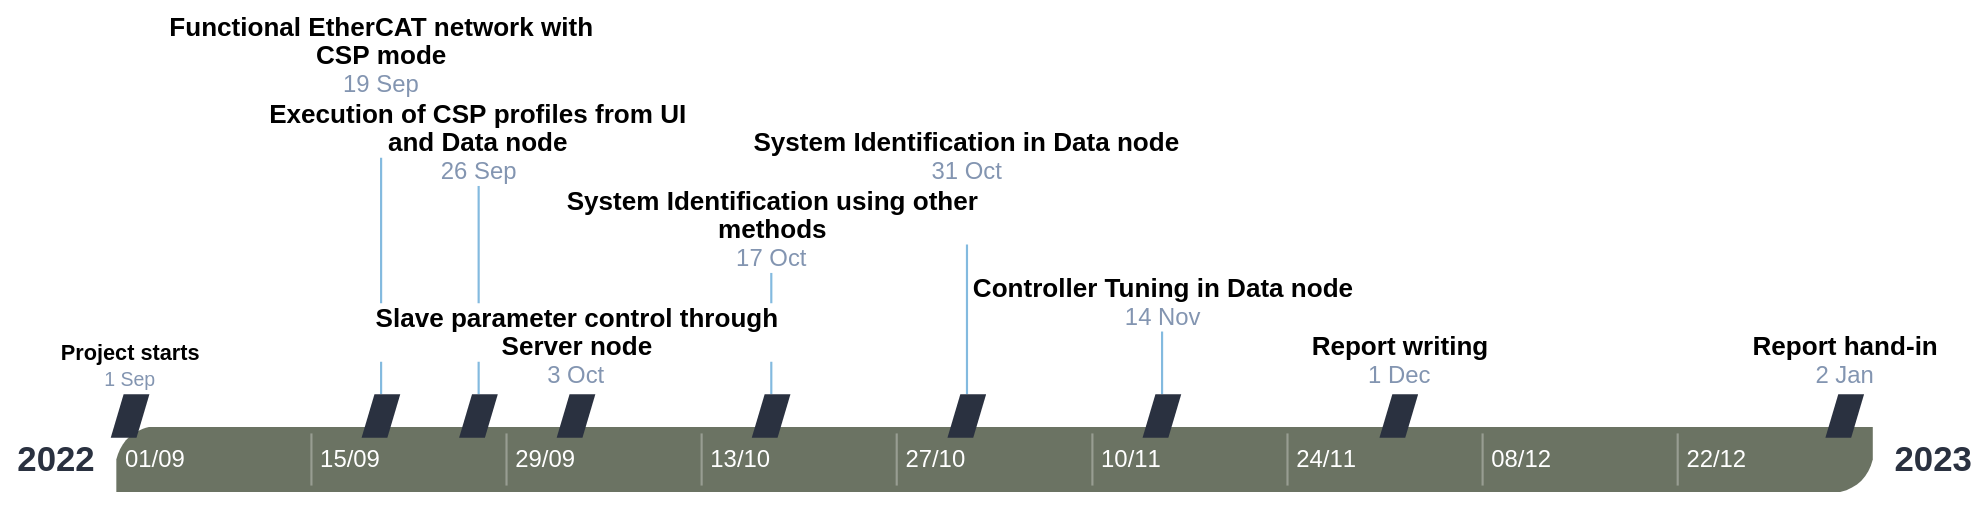
\includegraphics[width=\textwidth]{../resources/initial-description-timeline.png}
\end{center}

%This project will focus on extending and examining the functionality of the SOEM library inside a ROS2 environment. This will be achieved as a two phase process. 
%
%\textbf{Phase 1} will contain integrating the SOEM library into a ROS2 Node as a server-type EtherCAT management and control interface. Alongside, a supporting ESI schema parser which will expose drive capabilities to the EtherCAT server, and an RQt integrated control dashboard to allow user-friendly control over the network will be developed. 
%
%\textbf{Phase 2} will contain an examination of a specific EtherCAT servo drive, specifically extending the developed dashboard to be usable for parameter, friction, and system inertia estimation. To support the estimations, a demonstration of visual data presentation in a ROS-like manner is also included. 
%
%\subsection{Phase 1}
%\subsubsection{Description}
%
%\noindent
%Developing a ROS2 Node to serve as an EtherCAT Master using the SOEM library. The Node would be responsible for the following:  
%
%\vspace{6pt}
%\begin{itemize}[nosep]
%	\item Control of the EtherCAT Master FSM.
%	\item Control of each slave CiA-402 FSM.
%	\item Providing Messages, Actions, and Services on the ROS2 network from the EtherCAT network, to facilitate reading and writing EtherCAT network parameters. 
%\end{itemize}
%\vspace{6pt}
%
%\noindent
%Developing an RQt integrated dashboard for the EtherCAT server Node. It would provide the following:
%
%\vspace{6pt}
%\begin{itemize}[nosep]
%	\item Ability to send each specific state changing command to the network or specific slave.
%	\item Ability to select network or specific slave state and have it automatically change.
%	\item Ability to view the state of each part of the EtherCAT network.
%\end{itemize}
%\vspace{6pt}
%
%\noindent
%Developing a ROS2 ESI parser to provide the following:
%\vspace{6pt}
%\begin{itemize}[nosep]
%	\item Reading and parsing \textit{EtherCAT Slave Information} files.
%	\item Exposing the specific EtherCAT slave capabilities and information to the ROS2 network. 
%\end{itemize}
%\vspace{6pt}
%
%\subsubsection{Investigation}
%
%\vspace{6pt}
%\begin{itemize}[nosep]
%	\item How to achieve easy ROS2 integration of various EtherCAT drives compliant to CiA-402, including the device specific part of the profile.
%	\item How to fascilitate updating of EtherCAT network parameters through a ROS2 integrated interface. 
%\end{itemize}
%\vspace{6pt}
%
%\subsubsection{Experimentation} 
%
%\vspace{6pt}
%\begin{itemize}[nosep]
%	\item Connecting an EtherCAT device and verifying parsing Node results against manufacturer specifications. 
%	\item Setting and verifying network parameters through an RQt-based interface.
%\end{itemize}
%\vspace{6pt}
%
%\subsubsection{Components}
%
%\vspace{6pt}
%\begin{itemize}[nosep]
%	\item EtherCAT Server Node
%	\item RQt Network Dashboard
%	\item ESI Parser Node
%\end{itemize}
%\vspace{6pt}
%
%\subsection{Phase 2}
%\subsubsection{Description}
%
%\noindent
%Utilizing one of the synchronous motion profiles defined in CiA-402 for estimation of system parameters, including but perhaps not limited to the following:
%
%\vspace{6pt}
%\begin{itemize}[nosep]
%	\item Friction
%	\item System inertia
%	\item Resonance frequency
%\end{itemize}
%\vspace{6pt}
%
%\noindent
%This will also include presenting achieved and expected motions to the user though an RQt integrated interface, as well as relevant information related to the motion. 
%
%\subsubsection{Investigation}
%
%\vspace{6pt}
%\begin{itemize}[nosep]
%	\item How to quantify the quality of an achieved movement profile.
%	\item How to achieve parameter estimation using the CiA-402 standard and manufacturer specifications.
%	\item Determining an optimal motion for modal analysis. 
%\end{itemize}
%\vspace{6pt}
%
%\subsubsection{Experimentation}
%
%\vspace{6pt}
%\begin{itemize}[nosep]
%	\item Estimating friction in a known setup.
%	\item Estimating system inertia in a known setup. 
%	\item Frequency content analysis comparison for varying motion profiles and network cycle times.
%\end{itemize}
%\vspace{6pt}
%
%\subsubsection{Components}
%
%\vspace{6pt}
%\begin{itemize}[nosep]
%	\item Extending the developed EtherCAT Network Dashboard
%\end{itemize}
%\vspace{6pt}
